% Options for packages loaded elsewhere
\PassOptionsToPackage{unicode}{hyperref}
\PassOptionsToPackage{hyphens}{url}
%
\documentclass[
]{book}
\usepackage{lmodern}
\usepackage{amssymb,amsmath}
\usepackage{ifxetex,ifluatex}
\ifnum 0\ifxetex 1\fi\ifluatex 1\fi=0 % if pdftex
  \usepackage[T1]{fontenc}
  \usepackage[utf8]{inputenc}
  \usepackage{textcomp} % provide euro and other symbols
\else % if luatex or xetex
  \usepackage{unicode-math}
  \defaultfontfeatures{Scale=MatchLowercase}
  \defaultfontfeatures[\rmfamily]{Ligatures=TeX,Scale=1}
\fi
% Use upquote if available, for straight quotes in verbatim environments
\IfFileExists{upquote.sty}{\usepackage{upquote}}{}
\IfFileExists{microtype.sty}{% use microtype if available
  \usepackage[]{microtype}
  \UseMicrotypeSet[protrusion]{basicmath} % disable protrusion for tt fonts
}{}
\makeatletter
\@ifundefined{KOMAClassName}{% if non-KOMA class
  \IfFileExists{parskip.sty}{%
    \usepackage{parskip}
  }{% else
    \setlength{\parindent}{0pt}
    \setlength{\parskip}{6pt plus 2pt minus 1pt}}
}{% if KOMA class
  \KOMAoptions{parskip=half}}
\makeatother
\usepackage{xcolor}
\IfFileExists{xurl.sty}{\usepackage{xurl}}{} % add URL line breaks if available
\IfFileExists{bookmark.sty}{\usepackage{bookmark}}{\usepackage{hyperref}}
\hypersetup{
  pdftitle={Standar Pelayanan Minimal},
  pdfauthor={Registrasi Mahasiswa Universitas Sultan Ageng Tirtayasa Tahun 2020},
  hidelinks,
  pdfcreator={LaTeX via pandoc}}
\urlstyle{same} % disable monospaced font for URLs
\usepackage{longtable,booktabs}
% Correct order of tables after \paragraph or \subparagraph
\usepackage{etoolbox}
\makeatletter
\patchcmd\longtable{\par}{\if@noskipsec\mbox{}\fi\par}{}{}
\makeatother
% Allow footnotes in longtable head/foot
\IfFileExists{footnotehyper.sty}{\usepackage{footnotehyper}}{\usepackage{footnote}}
\makesavenoteenv{longtable}
\usepackage{graphicx}
\makeatletter
\def\maxwidth{\ifdim\Gin@nat@width>\linewidth\linewidth\else\Gin@nat@width\fi}
\def\maxheight{\ifdim\Gin@nat@height>\textheight\textheight\else\Gin@nat@height\fi}
\makeatother
% Scale images if necessary, so that they will not overflow the page
% margins by default, and it is still possible to overwrite the defaults
% using explicit options in \includegraphics[width, height, ...]{}
\setkeys{Gin}{width=\maxwidth,height=\maxheight,keepaspectratio}
% Set default figure placement to htbp
\makeatletter
\def\fps@figure{htbp}
\makeatother
\setlength{\emergencystretch}{3em} % prevent overfull lines
\providecommand{\tightlist}{%
  \setlength{\itemsep}{0pt}\setlength{\parskip}{0pt}}
\setcounter{secnumdepth}{5}
\usepackage{booktabs}
\usepackage{booktabs}
\usepackage{longtable}
\usepackage{array}
\usepackage{multirow}
\usepackage{wrapfig}
\usepackage{float}
\usepackage{colortbl}
\usepackage{pdflscape}
\usepackage{tabu}
\usepackage{threeparttable}
\usepackage{threeparttablex}
\usepackage[normalem]{ulem}
\usepackage{makecell}
\usepackage[]{natbib}
\bibliographystyle{apalike}

\title{Standar Pelayanan Minimal}
\author{Registrasi Mahasiswa Universitas Sultan Ageng Tirtayasa Tahun 2020}
\date{2020-11-09}

\begin{document}
\maketitle

{
\setcounter{tocdepth}{1}
\tableofcontents
}
\hypertarget{kata-pengantar}{%
\chapter*{KATA PENGANTAR}\label{kata-pengantar}}
\addcontentsline{toc}{chapter}{KATA PENGANTAR}

Penyempurnaan \textbf{Buku Standar Pelayanan Minimal} (\textbf{SPM}) Pelaksanaan Registrasi Mahasiswa tahun 2020 sesuai dengan perkembangan Ilmu dan Teknologi/IT dengan menggunakan e-administrasi (layanan administrasi akademik \emph{online}) Univeritas Sultan Ageng Tirtayasa, sebagai acuan dalam memberikan pelayanan dan informasi di Biro Akademik, Kemahasiswaan, dan Perencanaan (BAKP) terhadap mahasiswa Universitas Sultan Ageng Tirtayasa serta mempermudah mahasiswa dalam mengajukan permohonan registrasi (efesiensi waktu) sesuai kebutuhan mahasiswa.
Standar Pelayanan Minimal (SPM) Registrasi Mahasiswa ini merupakan penjabaran dari Pedoman Akademik, Program Kerja Universitas Sultan Ageng Tirtayasa tahun 2020, dan Program Kerja Biro Akademik, Kemahasiswaan, dan Perencanaan (BAKP) tahun 2020.

\textbf{Standar Pelayanan Minimal} (\textbf{SPM}) Registrasi Mahasiswan ini dasar pemikiran pelaksanaan administrasi \emph{online} (e-administrasi) agar dapat terpantau dan memiliki keseragaman kegiatan administrasi baik dalam proses maupun prosedur serta kebijakannya. Prinsip implementasi prosedur e-administrasi adalah :

\begin{enumerate}
\def\labelenumi{\arabic{enumi}.}
\tightlist
\item
  Memberikan pelayanan prima kepada mahasiswa,
\item
  Memberikan kepuasan terhadap layanan akademik terhadap mahasiswa,
\item
  Melakukan efesiensi penggunaan kertas dalam layanan akademik,
\item
  Penyergaman prosedur dan kebijakan dalam pelaksanaan layanan akademik,
\item
  Mendokumentasikan secara akurat proses layanan akademik mahasiswa. Pelaksanaan kegiatan registrasi mahasiswa di Universitas Sultan Ageng Tirtayasa sesuai dengan permasalahan pendidikan yang berkembang, maka Standar Pelayanan Minimal (SPM) Registrasi mahasiswa inipun terus dilakukan perbaikan dan penyempurnaan setiap waktu, sehingga sesuai dan selaras dengan kebutuhan dan dinamika perkembangan akademik.
\end{enumerate}

Kami berharap \textbf{Standar Pelayanan Minimal} (\textbf{SPM}) Registrasi Mahasiswa ini dapat berfungsi sebagai acuan dalam melaksanakan kegiatan registrasi mahasiswa baik pada tingkat Universitas, Fakultas, Jurusan atau Program Studi, Pimpinan, Mahasiswa, Dosen, dan Pegawai di lingkungan Universitas Sultan Ageng Tirtayasa.

Serang, April 2020\\
Kepala BAKP Untirta

\(~\)

Drs. Mochamad Ganiadi, M.M.\\
NIP. 19620422 199203 1 001

\hypertarget{intro}{%
\chapter{PENDAHULUAN}\label{intro}}

\hypertarget{latar-belakang}{%
\section{Latar Belakang}\label{latar-belakang}}

\textbf{Universitas Sultan Ageng Tirtayasa} dimulai dari Yayasan Pendidikan Tirtayasa (Yapenta) yang didirikan pada tanggal 1 Oktober 1980, Saat ini, Yapenta berubah menjadi Lapenta (Lembaga Pendidikan Tirtayasa). Yapenta berkedudukan dan bertempat di Kabupaten Serang. Pendirian Yapenta dikukuhkan dengan Akte Notaris Rosita Wibowo, SH, Nomor 1, tanggal 1 Oktober 1980. Kemudian dilakukan penyempurnaan dan dikukuhkan kembali dengan Akte Notaris Ny. R. Arie Soetardjo, Nomor 1, tanggal 3 Maret 1986.

Tujuan pendirian Yapenta adalah.

\begin{enumerate}
\def\labelenumi{\arabic{enumi}.}
\tightlist
\item
  Membantu usaha-usaha pemerintah dalam bidang pendidikan umum. Yaitu mulai dari taman kanak-kanak sampai dengan perguruan tinggi
\item
  Mendirikan sekolah-sekolah mulai dari taman kanak-kanak sampai dengan perguruan tinggi, termasuk juga sekolah-sekolah kejuruan.
\item
  Merencanakan dan mengusahakan sarana pendidikan, termasuk juga sarana olah raga.
\end{enumerate}

Kata Tirtayasa diambil dari nama pahlawan nasional yang berasal dari Banten, yaitu \textbf{Sultan Ageng Tirtayasa} (Kepres RI Nomor: 045/TK/1070). Nama asli Sultan Ageng Tirtayasa adalah Abul Fathi Abdul Fatah, pewaris kesultanan Banten keempat, yang dengan gigih menentang penjajahan Belanda dan berhasil membawa kejayaan dan keemasan Banten. Kata Tirtayasa sendiri berarti air mengalir (Sansekerta).

Pada awalnya Yayasan Pendidikan Tirtayasa (Yapenta) Banten menaungi Sekolah Tinggi Ilmu Hukum (STIH), Sekolah Tinggi Keguruan dan Ilmu Pendidikan (STKIP), dan Sekolah Tinggi Teknik (STT). STIH didirikan pada tanggal 1 Oktober 1980, sebagai embrio terbentuknya Universitas Tirtayasa (Untirta). Kemudian tanggal 1 Oktober 1980 disepakati sebagai tanggal kelahiran Untirta, sehingga upacara Dies Natalis Universitas Sultan Ageng Tirtayasa (Untirta) dilaksanakan tiap tanggal 1 Oktober.

Universitas Tirtayasa Banten merupakan penggabungan dari STIH, STT dan STKIP didasarkan pada SK Mendikbud RI Nomor:0596/0/1984, tanggal 28 Nopember 1984, ditingkatkan statusnya, sehingga menjadi Fakultas Hukum, Fakultas Teknik, dan Fakultas Ilmu Keguruan dan Pendidikan. Selanjutnya dengan SK Mendikbud RI Nomor: 0597/0/1984, tanggal 28 Nopember 1984, ketiga Fakultas tersebut ditetapkan sebagai status terdaftar.

Untirta berkembang dengan berdirinya Fakultas Pertanian dan Fakultas Ekonomi secara berturut-turut dengan SK Mendikbud RI Nomor: 0123/0/189, tanggal 8 Maret 1989, dan Nomor: 0331/0/1989, tanggal 30 Mei 1989, masing-masing dengan status terdaftar. Selanjutnya pada tanggal 13 Oktober 1999 keluar Keppres RI Nomor: 130/1999 tentang Persiapan Perguruan Tinggi Negeri Universitas Sultan Ageng Tirtayasa. Berdasarkan Keputusan Presiden RI Nomor: 32 tanggal 19 Maret 2001, Universitas Sultan Ageng Tirtayasa menjadi Perguruan Tinggi Negeri, maka Universitas Sultan Ageng Tirtayasa beralih dari naungan Yayasan Pendidikan Tirtayasa Banten (Yapenta) masuk kedalam lingkungan Departemen Pendidikan Nasional dan pengalihan aset serta pengelolaan sumber daya dari Yapenta kepada Pemerintah telah dilaksanakan. Tahun 2002.

Universitas Sultan Ageng Tirtayasa saat ini telah menyelenggarakan program pendidikan akademik dan program pendidikan vokasi. Program pendidikan akademik terdiri atas Program Pendidikan Sarjana (S1), Diploma (D3), sebanyaK enam fakultas dan satu program pendidikan Magister (Pascasarjana).

\hypertarget{fakultas-hukum}{%
\subsection{Fakultas Hukum}\label{fakultas-hukum}}

Memiliki satu jurusan/program studi strata satu (S1), yaitu : Ilmu Hukum kemudian berdasarkan keputusann Kemenristek Dikti nomor 257/M/KPT/2017 tentang nama program studi dan ditetapkan dengan SK Rektor Untirta Nomor 932/UN43/AK/SK/2017 menjadi Program Studi Hukum , dengan lima bidang studi yakni, Bidang Hukum Pidana, Bidang Hukum Perdata, Bidang Hukum Tata Negara, Bidang Hukum Administrasi Negara dan Bidang Hukum Internasional.

\hypertarget{fakultas-keguruan-dan-ilmu-pendidikan}{%
\subsection{Fakultas Keguruan dan Ilmu Pendidikan}\label{fakultas-keguruan-dan-ilmu-pendidikan}}

Memiliki 18 jurusan program strata satu (S1), mengalami penyesuaian berdasarkan Kemenristek Dikti nomor 257/M/KPT/2017 yaitu :

\begin{enumerate}
\def\labelenumi{\arabic{enumi}.}
\tightlist
\item
  Pendidikan Luar Sekolah (PLS) menjadi Pendidikan Nonformal,\\
\item
  Pendidikan Guru Sekolah Dasar (PGSD),
\item
  Pendidan Guru Pendidikan Anak usia Dini (PGPAUD),
\item
  Pendidikan Luar Biasa menjadi Pendidikan Khusus,
\item
  Bimbingan dan Konseling,
\item
  Pendidikan Bahasa dan Sastra Indonesia (Diksastrasia) menjadi Pendidikan Bahasa Indonesia,
\item
  Pendidikan Bahasa Inggris,
\item
  Pendidikan Seni Drama Tari dan Musik (Sendratasik) menjadi Pendidikan Seni Pertunjukan,
\item
  Pendidikan Matematika,
\item
  Pendidikan Biologi,
\item
  Pendidikan Fisika,
\item
  Pendidikan Kimia,
\item
  Pendidikan IPA,
\item
  Pendidikan Sejarah,
\item
  Pendidikan Pancasila dan Kewarganegaraan,
\item
  Pendidikan Sosiologi,
\item
  Pendidikan Teknik Elektro menjadi Pendidikan Vokasional Teknik Elektro,
\item
  Pendidikan Teknik Mesin menjadi Pendidikan Vokasional Teknik Mesin,
\end{enumerate}

\hypertarget{fakultas-teknik}{%
\subsection{Fakultas Teknik}\label{fakultas-teknik}}

Memiliki enam jurusan program strata satu (S1), yaitu:

\begin{enumerate}
\def\labelenumi{\arabic{enumi}.}
\tightlist
\item
  Teknik Mesin,\\
\item
  Teknik Elektro,\\
\item
  Teknik Industri,\\
\item
  Teknik Metalurgi,
\item
  Teknik Kimia,
\item
  Teknik Sipil.
\end{enumerate}

\hypertarget{fakultas-pertanian}{%
\subsection{Fakultas Pertanian}\label{fakultas-pertanian}}

Memiliki tiga jurusan program strata satu (S1), yaitu:

\begin{enumerate}
\def\labelenumi{\arabic{enumi}.}
\tightlist
\item
  Agribisnis,\\
\item
  Agroekoteknologi,\\
\item
  Perikanan,
\item
  Teknologi Pangan.
\end{enumerate}

\hypertarget{fakultas-ekonomi-dan-bisnis}{%
\subsection{Fakultas Ekonomi dan Bisnis}\label{fakultas-ekonomi-dan-bisnis}}

Memiliki empat jurusan program strata satu (S1) dan empat program studi Diploma (D3), mengalami penyesuaian berdasarkan Kemenristek Dikti nomor 257/M/KPT/2017, yaitu:

\begin{enumerate}
\def\labelenumi{\arabic{enumi}.}
\tightlist
\item
  Manajemen,
\item
  Akuntansi,
\item
  Ekonomi Studi Pembangunan,
\item
  Ekonomi Islam menjadi Ekonomi Syariah
\item
  Akuntansi (D3),\\
\item
  Marketing (D3) menjadi Manajemen Pemasaran,\\
\item
  Perpajakan (D3),
\item
  Keuangan dan Perbankan (D3) menjadi Perbankan dan Keuangan.
\end{enumerate}

\hypertarget{fakultas-ilmu-sosial-dan-ilmu-politik}{%
\subsection{Fakultas Ilmu Sosial dan Ilmu Politik}\label{fakultas-ilmu-sosial-dan-ilmu-politik}}

Memiliki tiga jurusan program strata satu (S1), yaitu:

\begin{enumerate}
\def\labelenumi{\arabic{enumi}.}
\tightlist
\item
  Ilmu Administrasi Negar menjadi Administrasi Publik,\\
\item
  Ilmu Komunikasi,
\item
  Ilmu Pemerintahan.
\end{enumerate}

\hypertarget{fakultas-kedokteran}{%
\subsection{Fakultas Kedokteran}\label{fakultas-kedokteran}}

Memiliki tiga jurusan program strata satu (S1) dan satu program studi Diploma (D3), yaitu:

\begin{enumerate}
\def\labelenumi{\arabic{enumi}.}
\tightlist
\item
  Kedokteran
\item
  Gizi
\item
  Ilmu Keolahragaan
\item
  Keperawatan (D3)
\end{enumerate}

\hypertarget{pascasarjana}{%
\subsection{Pascasarjana}\label{pascasarjana}}

Memiliki program Magister strata dua (S2) dengan enam program studi, yaitu:

\begin{enumerate}
\def\labelenumi{\arabic{enumi}.}
\tightlist
\item
  Pendidikan Bahasa Indonesia,
\item
  Teknologi Pendidikan,
\item
  Hukum,
\item
  Magister Akuntansi,
\item
  Magister Manajemen,
\item
  Magister Administrasi Publik.
\item
  Pendidikan Bahasa Inggris,
\item
  Pendidikan Matematika,
\item
  Ilmu Pertanian.
\item
  Teknik Kimia
\item
  Ilmu Komunikasi
\end{enumerate}

\hypertarget{visi-misi-tujuan-sasaran-dan-strategi-universitas-sultan-ageng-tirtayasa}{%
\section{Visi, Misi, Tujuan, Sasaran, dan Strategi Universitas Sultan Ageng Tirtayasa}\label{visi-misi-tujuan-sasaran-dan-strategi-universitas-sultan-ageng-tirtayasa}}

\hypertarget{visi-universitas-sultan-ageng-tirtayasa}{%
\subsection{Visi Universitas Sultan Ageng Tirtayasa}\label{visi-universitas-sultan-ageng-tirtayasa}}

\begin{quote}
``Terwujudnya UNTIRTA Sebagai Integrated, Smart, and Green (It'S Green) University yang UNGGUL, BERKARAKTER, DAN BERDAYA SAING, di Kawasan ASEAN tahun 2030''
\end{quote}

Berdasarkan visi tersebut di atas dapat dijelaskan antara lain sebagai berikut:

\begin{enumerate}
\def\labelenumi{\arabic{enumi}.}
\item
  \textbf{Maju}. Mengandung pengertian terwujudnya kondisi Untirta yang mengalami pertumbuhan, peningkatan dan perubahan secara berkelanjutan dalam penyelenggaraan pendidikan dan pembelajaran, penelitian, dan pengabdian kepada masyarakat, daya dukung sumber daya dan manajemen serta kerjasama kemitraan.
\item
  \textbf{Bermutu}. Mengandung pengertian tercapainya kualitas layanan yang memberikan kepuasan kepada pelanggan, lulusan Universitas Sultan Ageng Tirtayasa yang menguasai Iptek (hard skill), mampu berkolaborasi dan membangun jejaring (networking) berkomunkasi (soft skill) menuju kemajuan bangsa, peradaban dan kesejahteraan umat manusia.
\item
  \textbf{Berdaya Saing}. Mengandung pengertian terwujudnya suatu dorongan pada diri pendidik (dosen, tenaga kependidikan, dan lulusan untuk memenangkan suatu persaingan (kompetisi), lebih berprestasi, memiliki keunggulan komparatif dan keunggulan kompetitif, berupaya lebih baik dari yang lain, tahan menghadapi berbagai kondisi, hambatan dan tantangan serta mampu beradaptasi dengan lingkungan.
\item
  \textbf{Berkarakter}. Mengandung arti tercapainya tenaga pendidik dan kependidikan serta lulusan universitas Sultan Ageng Tirtayasa yang menguasai Iptek dengan menjunjung tinggi kejujuran, amanah, berwibawa, adil, religius, dan akuntabel.
\item
  \textbf{Kebersamaan}. Dalam mewujudkan misi Untirta perlu terbangun komunikasi kerja di Universitas Sultan Ageng Tirtayasa lebih mengutamakan semangat gotong royong, kolegial, saling pengertian, saling menghargai dan saling menghormati, sebagai sebuah Tim kerja yang menjunjung tinggi solidaritas dan soliditas. Hal ini meniscayakan seluruh komponen Untirta mulai dari level teratas sampai dengan level terbawah bersama-sama berkomitmen memberikan.
\end{enumerate}

\hypertarget{misi-universitas-sultan-ageng-tirtayasa}{%
\subsection{Misi Universitas Sultan Ageng Tirtayasa}\label{misi-universitas-sultan-ageng-tirtayasa}}

Untuk mencapai Visi di atas, Universitas Sultan Ageng Tirtayasa menetapkan misi sebagai berikut:

\begin{enumerate}
\def\labelenumi{\arabic{enumi}.}
\tightlist
\item
  Meningkatkan kualitas, relevansi dan daya saing pendidikan serta lulusan yang unggul, berkarakter, serta berdaya saing di kawasan ASEAN.
\item
  Meningkatkan kualitas dan kuantitas penelitian dan pengabdian kepada masyarakat yang inovatif berbasis kebutuhan nyata sesuai perkembangan zaman.
\item
  Meningkatkan daya dukung tatakelola perguruan tinggi yang baik sebagai implementasi dari Integrated Smart and Green (It'S Green) University.
\end{enumerate}

\hypertarget{tujuan-universitas-sultan-ageng-tirtayasa}{%
\subsection{Tujuan Universitas Sultan Ageng Tirtayasa}\label{tujuan-universitas-sultan-ageng-tirtayasa}}

\begin{enumerate}
\def\labelenumi{\arabic{enumi}.}
\tightlist
\item
  Menghasilkan lulusan yang berkualitas, terdidik, terlatih, berdaya saing, dan berkarakter sesuai kebutuhan \emph{stakeholders}.
\item
  Menghasilkan penelitan dan pengabdian kepada masyarakat yang inovatif berbasis kebutuhan nyata serta berorientasi pada pemanfaatan oleh dunia industri, pembangunan daerah, dan masyarakat.
\item
  Menghasilkan daya dukung tatakelola yang efektif, efisien, transparan, dan akuntabel dalam mengembangkan tri dharma perguruan tinggi.
\end{enumerate}

\hypertarget{sasaran}{%
\subsection{Sasaran}\label{sasaran}}

Dalam rangka mencapai tujuan tersebut, perlu ditetapkan sasaran sebagai berikut:

\begin{enumerate}
\def\labelenumi{\arabic{enumi}.}
\tightlist
\item
  Meningkatnya kualitas, kuantitas, relevansi, dan daya saing lulusan.
\item
  Meningkatnya kualitas dan kuantitas Program Studi sesuai Kebutuhan \emph{Stakeholders}.
\item
  Meningkatnya kualitas dan kuantitas penelitian dan pengabdian kepada masyarakat.
\item
  Tersedianya daya dukung SDM sesuai Standar Kompetensi.
\item
  Meningkatnya daya dukung administrasi akademik dan non akademik.
\item
  Tersedianya daya dukung sarana prasarana yang memadai.
\item
  Kerjasama kemitraaan strategis nasional dan internasional.
\end{enumerate}

\hypertarget{strategi}{%
\subsection{Strategi}\label{strategi}}

\begin{enumerate}
\def\labelenumi{\arabic{enumi}.}
\tightlist
\item
  Penguatan Kualitas Layanan Pendidikan dan Organisasi Kemahasiswaan.
\item
  Penguatan Program Studi (akademik, vokasi, dan profesi) memenuhi standar Mutu Pendidikan Tinggi.
\item
  Penguatan Penelitian dan Pengabdian kepada Masyarakat yang inovatif berbasis kebutuhan industri, pembangunan daerah, dan masyarakat.
\item
  Penguatan SDM dosen dan tenaga kependidikan sesuai kompetensi.
\item
  Penguatan layanan administasi akademik dan nonakademik.
\item
  Penguatan Sarana dan prasarana perguruan tinggi.
\item
  Penguatan Kerjasama dan kemitraan.
\end{enumerate}

\hypertarget{pendidikan-tinggi}{%
\section{Pendidikan Tinggi}\label{pendidikan-tinggi}}

Program pendidikan tinggi yang diselenggarakan oleh Universitas Sultan Ageng Tirtayasa: (1) Program Pendidikan Akademik, (2) Program Pendidikan Vokasi. Adapun pengertiannya adalah sebagai berikut:

\hypertarget{program-pendidikan-akademik}{%
\subsection{Program Pendidikan Akademik}\label{program-pendidikan-akademik}}

Bertujuan menyiapkan peserta didik untuk menjadi anggota masyarakat yang memiliki kemampuan akademik dalam menerapkan, mengembangkan, dan/atau memperkaya khasanah ilmu pengetahuan, teknologi, dan/atau kesenian, serta menyebarluaskan dan mengupayakan penggunaannya untuk meningkatkan taraf kehidupan masyarakat dan memperkaya kebudayaan nasional. Program pendidikan akademik di Untirta terdiri atas Program Sarjana (S1) dan Program Pascasarjana (S2).

\hypertarget{tujuan-pendidikan-program-magister}{%
\subsubsection{Tujuan Pendidikan Program Magister}\label{tujuan-pendidikan-program-magister}}

Program Magister diarahkan pada hasil lulusan yang memiliki kualifikasi sebagai berikut:

\begin{enumerate}
\def\labelenumi{\arabic{enumi}.}
\tightlist
\item
  Mampu menguasai perkembangan ilmu pengetahuan, teknologi,dan/atau seni dalam bidangnya dengan cara menguasai dan memahami teori-teori yang mutakhir, pendekatan, metode, dan kaidah-kaidah ilmiah disertai penerapannya.
\item
  Mampu memecahkan permasalahan di bidang keahliannya melalui kegatan penelitian dan pengembangan berdasarkan kaidah ilmiah.
\item
  Mampu mengembangkan kinerja profesionalnya yang ditunjukkan dengan ketajaman analisis permasalahan dan kepaduan pemecahan masalah.
\item
  Mampu berkomunikasi efektif termasuk berbahasa internasional.
\end{enumerate}

\hypertarget{tujuan-program-sarjana}{%
\subsubsection{Tujuan Program Sarjana}\label{tujuan-program-sarjana}}

Program Sarjana diarahkan pada hasil lulusan yang memiliki kualifikasi sebagai berikut:

\begin{enumerate}
\def\labelenumi{\arabic{enumi}.}
\tightlist
\item
  Menguasai dasar-dasar ilmiah dan keterampilan dalam bidang keahlian tertentu sehingga mampu menemukan, memahami, menjelaskan, dan merumuskan cara penyelesaian masalah yang ada di dalam kawasan keahliannya.
\item
  Mampu menerapkan ilmu pengetahuan dan keterampilan yang dimilikinya sesuai dengan bidang keahliannya dalam kegiatan produktif dan pelayanan kepada masyarakat dengan sikap dan perilaku yang sesuai dengan tata kehidupan bermasyarakat.
\item
  Mampu bersikap dan berperilaku dalam membawa diri berkarya di bidang keahliannya maupun dalam kehidupan bersama dalam masyarakat.
\item
  Mampu mengikuti perkembangan ilmu pengetahuan, teknologi, dan/atau kesenian yang merupakan keahliannya.
\item
  Mampu bersaing dan beradaptasi dalam lingkungan persaingan global.
\end{enumerate}

\hypertarget{program-pendidikan-vokasi}{%
\subsection{Program Pendidikan Vokasi}\label{program-pendidikan-vokasi}}

Bertujuan menyiapkan peserta didik menjadi anggota masyarakat yang memiliki pengetahuan dan keterampilan di bidang kerja serta memiliki tanggungjawab profesional terhadap pekerjaannya, serta mampu melaksanakan pengawasan dan bimbingan atas dasar keterampilan manajerial yang dimilikinya. Program pendidikan vokasional yang diselenggarakan adalah Program Diploma III.

\hypertarget{tujuan-pendidikan-program-vokasi}{%
\subsubsection{Tujuan Pendidikan Program Vokasi}\label{tujuan-pendidikan-program-vokasi}}

Program vokasi diarahkan untuk menghasilkan tenaga ahli madya yang memiliki kualifikasi sebagai berikut:

\begin{enumerate}
\def\labelenumi{\arabic{enumi}.}
\tightlist
\item
  Mampu menguasai perkembangan ilmu pengetahuan, teknologi, dan/atau seni dalam bidangnya kearah kegiatan yang produktif.
\item
  Terampil dan profesional kearah pemecahan masalah serta pelayanan langsung kepada masyarakat sesuai dengan bidang keahliannya.
\item
  Memiliki integritas kepribadian yang tinggi serta berjiwa entrepreneurial.
\end{enumerate}

\textbf{Program Studi, Kode Fakultas, dan Kode Jurusan/Program Studi Universitas Sultan Ageng Tirtayasa}

\begin{enumerate}
\def\labelenumi{\arabic{enumi}.}
\tightlist
\item
  Program Pascasarjana (S2)
\end{enumerate}

\begin{longtable}{c|l|c|c}
\hline
\multicolumn{2}{c|}{ } & \multicolumn{2}{c}{Kode} \\
\cline{3-4}
No & Program Studi & Fakultas & Program Studi\\
\hline
\endfirsthead
\multicolumn{4}{@{}l}{\textit{(continued)}}\\
\hline
No & Program Studi & Fakultas & Program Studi\\
\hline
\endhead
1 & Pendidikan Bahasa Indonesia & 77 & 71\\
\hline
2 & Teknologi Pendidikan & 77 & 72\\
\hline
3 & Hukum & 77 & 73\\
\hline
4 & Magister Akuntansi & 77 & 74\\
\hline
5 & Magister Administrasi Publik & 77 & 75\\
\hline
6 & Magister Manajemen & 77 & 76\\
\hline
7 & Pendidikan Bahasa Inggris & 77 & 77\\
\hline
8 & Pendidikan Matematika & 77 & 78\\
\hline
9 & Ilmu Pertanian & 77 & 79\\
\hline
10 & Teknik Kimia & 77 & 80\\
\hline
11 & Ilmu Komunikasi & 77 & 81\\
\hline
12 & Pendidikan (S3) & 77 & 82\\
\hline
\end{longtable}

\begin{enumerate}
\def\labelenumi{\arabic{enumi}.}
\setcounter{enumi}{1}
\tightlist
\item
  Program Sarjana (S1)
\end{enumerate}

\begin{longtable}{l|c|c}
\hline
\multicolumn{1}{c|}{ } & \multicolumn{2}{c}{Kode} \\
\cline{2-3}
Fakultas/Program Studi & Fakultas & Program Studi\\
\hline
\endfirsthead
\multicolumn{3}{@{}l}{\textit{(continued)}}\\
\hline
Fakultas/Program Studi & Fakultas & Program Studi\\
\hline
\endhead
\multicolumn{3}{l}{\textbf{Hukum}}\\
\hline
\hspace{1em}Hukum & 11 & 11\\
\hline
\multicolumn{3}{l}{\textbf{Keguruan dan Ilmu Pendidikan}}\\
\hline
\hspace{1em}Pendidikan Nonformal & 22 & 21\\
\hline
\hspace{1em}Pendidikan Bahasa Indonesia & 22 & 22\\
\hline
\hspace{1em}Pendidikan Bahasa Inggris & 22 & 23\\
\hline
\hspace{1em}Pendidikan Biologi & 22 & 24\\
\hline
\hspace{1em}Pendidikan Matematika & 22 & 25\\
\hline
\hspace{1em}Pendidikan Guru Sekolah Dasar & 22 & 27\\
\hline
\hspace{1em}Pendidikan Guru Pendidikan Anak Usia Dini & 22 & 28\\
\hline
\hspace{1em}Pendidikan Fisika & 22 & 80\\
\hline
\hspace{1em}Pendidikan IPA & 22 & 81\\
\hline
\hspace{1em}Pendidikan Kimia & 22 & 82\\
\hline
\hspace{1em}Pendidikan (Vokasional) Teknik Elektro & 22 & 83\\
\hline
\hspace{1em}Pendidikan (Vokasional) Teknik Mesin & 22 & 84\\
\hline
\hspace{1em}Bimbingan dan Konseling & 22 & 85\\
\hline
\hspace{1em}Pendidikan Pancasila dan Kewarganegraan & 22 & 86\\
\hline
\hspace{1em}Pendidikan Khusus & 22 & 87\\
\hline
\hspace{1em}Pendidikan Sejarah & 22 & 88\\
\hline
\hspace{1em}Pendidikan Seni Pertunjukan & 22 & 89\\
\hline
\hspace{1em}Pendidikan Sosiologi & 22 & 90\\
\hline
\multicolumn{3}{l}{\textbf{Teknik}}\\
\hline
\hspace{1em}Teknik Mesin & 33 & 31\\
\hline
\hspace{1em}Teknik Elektro & 33 & 32\\
\hline
\hspace{1em}Teknik Industri & 33 & 33\\
\hline
\hspace{1em}Teknik Metalurgi & 33 & 34\\
\hline
\hspace{1em}Teknik Kimia & 33 & 35\\
\hline
\hspace{1em}Teknik Sipil & 33 & 36\\
\hline
\multicolumn{3}{l}{\textbf{Pertanian}}\\
\hline
\hspace{1em}Agribisnis & 44 & 41\\
\hline
\hspace{1em}Agroekoteknologi & 44 & 42\\
\hline
\hspace{1em}Perikanan & 44 & 43\\
\hline
\hspace{1em}Teknologi Pangan & 44 & 44\\
\hline
\multicolumn{3}{l}{\textbf{Ekonomi dan Bisnis}}\\
\hline
\hspace{1em}Manajemen & 55 & 51\\
\hline
\hspace{1em}Akuntansi & 55 & 52\\
\hline
\hspace{1em}Ekonomi Pembangunan & 55 & 53\\
\hline
\hspace{1em}Ekonomi Syariah & 55 & 54\\
\hline
\multicolumn{3}{l}{\textbf{Ilmu Sosial dan Ilmu Politik}}\\
\hline
\hspace{1em}Administrasi Publik & 66 & 61\\
\hline
\hspace{1em}Ilmu Komunikasi & 66 & 62\\
\hline
\hspace{1em}Ilmu Pemerintahan & 66 & 70\\
\hline
\multicolumn{3}{l}{\textbf{Kedokteran}}\\
\hline
\hspace{1em}Kedokteran & 88 & 81\\
\hline
\hspace{1em}Gizi & 88 & 82\\
\hline
\hspace{1em}Ilmu Keolahragaan & 88 & 83\\
\hline
\end{longtable}

\begin{enumerate}
\def\labelenumi{\arabic{enumi}.}
\setcounter{enumi}{2}
\tightlist
\item
  Program Diploma (D3)
\end{enumerate}

\begin{longtable}{l|c|c}
\hline
\multicolumn{1}{c|}{ } & \multicolumn{2}{c}{Kode} \\
\cline{2-3}
Fakultas/Program Studi & Fakultas & Program Studi\\
\hline
\endfirsthead
\multicolumn{3}{@{}l}{\textit{(continued)}}\\
\hline
Fakultas/Program Studi & Fakultas & Program Studi\\
\hline
\endhead
\multicolumn{3}{l}{\textbf{Ekonomi dan Bisnis}}\\
\hline
\hspace{1em}Akuntansi & 55 & 01\\
\hline
\hspace{1em}Manajemen Pemasaran & 55 & 02\\
\hline
\hspace{1em}Perpajakan & 55 & 03\\
\hline
\hspace{1em}Perbankan dan Keuangan & 55 & 04\\
\hline
\multicolumn{3}{l}{\textbf{Kedokteran}}\\
\hline
\hspace{1em}Keperawatan & 88 & 01\\
\hline
\end{longtable}

\begin{center}\rule{0.5\linewidth}{0.5pt}\end{center}

\begin{center}\rule{0.5\linewidth}{0.5pt}\end{center}

\hypertarget{registrasi-mahasiswa-baru}{%
\chapter{REGISTRASI MAHASISWA BARU}\label{registrasi-mahasiswa-baru}}

Registrasi merupakan prosedur awal bagi mahasiswa baru Universitas Sultan Ageng Tirtayasa. Mahasiswa Universitas Sultan Ageng Tirtayasa adalah mahasiswa yang telah menyelesaikan ketentuan dan prosedur yang berlaku. Pada prosesnya prosedur ini melibatkan 6 (enam) entitas, yaitu:

\begin{enumerate}
\def\labelenumi{\arabic{enumi}.}
\tightlist
\item
  Mahasiswa.
\item
  Subbagian Registrasi \& Statistik/BAKP.
\item
  Subbagian Kemahasiswaan/BAKP.
\item
  Subbagian PNBP/BUKK.
\item
  Pusat Data dan Informasi (PUSDAINFO).
\item
  Jurusan/Program Studi/Fakultas/Pascasarjana.
\end{enumerate}

\hypertarget{ketentuan-mahasiswa-baru}{%
\section{Ketentuan Mahasiswa Baru}\label{ketentuan-mahasiswa-baru}}

Bagi calon mahasiswa baru sudah \textbf{\emph{lulus tes seleksi}} / ujian masuk perguruan tinggi di Universitas Sultan Ageng Tirtayasa melalui beberapa jalur masuk : Seleksi Nasional Masuk Perguruan Tinggi Negeri (SNMPTN) dengan Program Sarjana (S1), Seleksi Bersama Masuk Perguruan Tinggi Negeri (SBMPTN) dengan Program Sarjana (S1), Seleksi Masuk Mandiri Perguruan Tinggi Negeri (SMMPTN) dengan Program Sarjana (S1), Ujian Masuk Mandiri (UMM) dengan Program Diploma (D3) dan Seleksi Penerimaan Mahasiswa Baru (SPMB) dengan Program Magister (S2/S3) diselenggarakan oleh Pascasarjana Universitas Sultan Ageng Tirtayasa.

Setelah lulus seleksi bukti lulusnya dituangkan dalam dokumen Surat Keputusan Rektor Universitas Sultan Ageng Tirtayasa tentang hasil seleksi penerimaan mahasiswa baru dari beberapa jalur masuk yang diterbitkan pada tahun akademik oleh Universitas Sultan Ageng Tirtayasa.

Selanjutnya calon mahasiswa melengkapi persyaratan administrasi akademik dan administrasi keuangan / sudah membayar Uang Kuliah Tunggal (UKT)/ Sumbangan Pengembangan Pendidikan (SPP) bagi mahasiswa baru Program Sarjana (S1) dan Program Diploma (D3) dan calon mahasiswa melengkapi persyaratan administrasi akademik dan administrasi keuangan serta sudah membayar Sumbangan Pengembangan Pendidikan (SPP) bagi mahasiswa baru Program Magister (S2/S3).

Bagi mahasiswa baru baik Program Sarjana (S1) dan Program Diploma (D3) melakukan registrasi akademik dengan melengkapi persyaratan dan ketentuan yang telah ditetapkan.

\hypertarget{waktu-registrasi}{%
\section{Waktu Registrasi}\label{waktu-registrasi}}

Pelaksanaan registrasi mahasiswa baru mengacu pada ketentuan yang telah di tuangkan dalam kalender akademik pada semester gasal (Program Sarjana (S1) dan Diploma (D3), semester gasal dan genap (Program Magister (S2)) sehingga mahasiswa sudah punya dasar dan gambaran yang pasti akan waktu pelaksanaan kegiatan Registrasi Mahasiswa Baru tersebut dan proses perkuliahan dapat berjalan dengan baik.

\hypertarget{prosedur-persyaratan-mahasiswa-baru}{%
\section{Prosedur Persyaratan Mahasiswa Baru}\label{prosedur-persyaratan-mahasiswa-baru}}

\hypertarget{mahasiswa-baru}{%
\subsection{Mahasiswa Baru}\label{mahasiswa-baru}}

Calon mahasiswa melihat informasi ke \url{http://admisi.untirta.ac.id},

\begin{enumerate}
\def\labelenumi{\alph{enumi}.}
\tightlist
\item
  Surat Keputusan Rektor Tentang Hasil Seleksi Mahasiswa Baru sesuai dengan jalur masuk SNMPTN, SBMPTN, SMMPTN, UMM.
\item
  Pengumuman Registrasi mahasiswa baru sesuai dengan jalur masuk SNMPTN, SBMPTN, SMMPTN, UMM.
\item
  Alur Registrasi Mahasiswa Baru sesuai dengan jalur masuk SNMPTN, SBMPTN, SMMPTN, UMM.
\end{enumerate}

\hypertarget{pengisianpengambilan-persyaratan-berkas-registrasi}{%
\subsection{Pengisian/Pengambilan Persyaratan Berkas Registrasi}\label{pengisianpengambilan-persyaratan-berkas-registrasi}}

Calon Mahasiswa Baru \emph{login} ke \url{http://admisi.untirta.ac.id}, dengan \emph{username}: Nomor Peserta SNMPTN, SBMPTN, SMMPTN, UMM serta \emph{password}: Tanggal Lahir.

\begin{enumerate}
\def\labelenumi{\alph{enumi}.}
\tightlist
\item
  Pengisian Biodata Mahasiswa dan mengunggah Foto terbaru (latar belakang merah dan memakai kemeja putih).
\item
  Mengunduh Pakta Integritas Uang Kuliah Tunggal (UKT)/Biaya Pendidikan
\item
  Mengunduh dan Surat Pernyataan Mentaati Peraturan Untirta
\end{enumerate}

\hypertarget{data-pendukung-lampiran-berkas-registrasi}{%
\subsection{Data Pendukung Lampiran Berkas Registrasi}\label{data-pendukung-lampiran-berkas-registrasi}}

Calon Mahasiswa Baru setelah melengkapi persyaratan, \emph{login} kembali ke \url{http://admisi.untirta.ac.id} dan kemudian \textbf{WAJIB} mengunggah seluruh persyaratan tanpa terkecuali antara lain:

\begin{enumerate}
\def\labelenumi{\alph{enumi}.}
\item
  Hasil pindah (\emph{scan}) Kartu Peserta SNMPTN, SBMPTN, SMMPTN, UMM.
\item
  Hasil pindai Ijazah atau SKHUN atau Surat Keterangan Lulus (SKL) bagi yang belum keluar ijasahnya.
\item
  Hasil pindai Tes Kesehatan
\item
  Hasil pindai Tes Narkoba
\item
  Hasil pindai Tes Buta Warna bagi jurusan tertentu:

  \begin{enumerate}
  \def\labelenumii{\arabic{enumii}.}
  \tightlist
  \item
    \textbf{FKIP} : Penddikan Biologi, Pendidikan Kimia, Pendidikan Fisika, Pendidikan IPA, Pendidikan Teknik Elektro, Pendidikan Teknik Mesin. PAUD.
  \item
    \textbf{Fakultas Teknik} : Teknik Kimia, Teknik Metalurgi, Teknik Mesin, Teknik Elektro.
  \item
    \textbf{Fakultas Pertanian} : Agribisnis, Agroekoteknologi, Perikanan, Teknologi Pangan.
  \item
    \textbf{Fakultas Kedokteran} : Keperawatan (D3).
  \end{enumerate}
\item
  Hasil pindai Akte Kelahiran.
\item
  Hasil pindai Tagihan Rekening Listrik Bulan terbaru dan tahun berjalan
\item
  Hasil pindai Pajak Bumi dan Bagunan (PBB) terbaru.
\item
  Hasil pindai Kartu Keluarga (KK).
\item
  Hasil pindai Slip Pengasilan orang tua bagi calon mahasiswa yang orang tuanya bekerja sebagai PNS/Swasta, yang ditanda-tangani oleh pejabat/pimpinan instansi tempat kerja, atau Hasil pindai Surat Keterangan Penghasilan yang ditandatangani oleh kelurahan atau kecamatan, jika orang tua bekerja sebagai Wiraswasta / Pedagang / Buruh / Petani / Pensiunan. (Jika kedua orang tua bekerja).
\end{enumerate}

\hypertarget{verifikasi-data-registrasi-oleh-subbagian-registrasi-dan-statistik-terhadap-data-yang-telah-diunggah-oleh-calon-mahasiswa-baru}{%
\subsection{Verifikasi data registrasi oleh Subbagian Registrasi dan Statistik terhadap data yang telah diunggah oleh calon mahasiswa baru}\label{verifikasi-data-registrasi-oleh-subbagian-registrasi-dan-statistik-terhadap-data-yang-telah-diunggah-oleh-calon-mahasiswa-baru}}

Tim dari Subbagian Registrasi dan statitik akan memeriksa data yang telah diunggah. Apabila data yang diunggah tidak lengkap maka tim akan menghubungi calon mahasiwa baru tersebut. Data ini diperlukan untuk menentukan dasar penentuan besaran UKT calon mahasiswa baru

\hypertarget{pengisianpengambilan-persyaratan-berkas-registrasi-program-magister-s2}{%
\subsection{Pengisian/Pengambilan Persyaratan Berkas Registrasi Program Magister (S2)}\label{pengisianpengambilan-persyaratan-berkas-registrasi-program-magister-s2}}

Calon Mahasiswa Baru pengambilan persyaratan di Subbagian Akademik Pascasarjana, Universitas Sultan Ageng Tirtayasa. Persyaratan yang harus dilengkapi calon mahasiswa baru:

\begin{enumerate}
\def\labelenumi{\alph{enumi}.}
\tightlist
\item
  Kartu Tanda Peserta Ujian SPMB
\item
  Pengisian Biodata Mahasiswa.
\item
  Ijazah S1, Akta IV (bagi yang memiliki AKTA IV) dan Transkrip Akademik di legalisir/Surat Keterangan Lulus asli bagi yang belum keluar Ijazah, Akta IV dan Transkrip Akademik.
\item
  Slip Pembayaran SPP.\\
\item
  Pas Photo terbaru berwarna (ukuran: 3x4): 2 Lembar.
\end{enumerate}

\hypertarget{biro-akademik-kemahasiswaan-dan-perencanaan-bakp}{%
\section{Biro Akademik, Kemahasiswaan, dan Perencanaan (BAKP)}\label{biro-akademik-kemahasiswaan-dan-perencanaan-bakp}}

\hypertarget{subbagian-registrasi-dan-statistik-memverifikasi-berkas-registrasi-mahasiswa-baru}{%
\subsection{Subbagian Registrasi dan Statistik memverifikasi Berkas Registrasi Mahasiswa Baru}\label{subbagian-registrasi-dan-statistik-memverifikasi-berkas-registrasi-mahasiswa-baru}}

\hypertarget{program-sarjana-s1-dan-diploma-d3}{%
\subsubsection{Program Sarjana (S1) dan Diploma (D3)}\label{program-sarjana-s1-dan-diploma-d3}}

Bagi calon mahasiswa setelah melakukan pengisian / pengambilan persyaratan registrasi secara \emph{online} (mengunduh dan mengunggah), persyaratan poin 3 nomor 3.1. -- 3.6 dan 3.12 -- 3.13 dibawa untuk dicek kebenarannya (membawa persyaratan asli) Ke Subbagian Registrasi dan Statistik, Biro Akademik, Kemahasiswaan dan Perencanaan (BAKP).

\hypertarget{program-magister-s2}{%
\subsubsection{Program Magister (S2)}\label{program-magister-s2}}

Bagi calon mahasiswa setelah melakukan pengisian/pengambilan persyaratan dan sudah melengkapi persyaratan registrasi diserahkan ke Subbagian Akademik Pascasarjana, berkas persayaratan tersebut secara kolektif oleh Subbagian Akademik Pascasarjana di serahkan ke Subbagian Registrasi dan Statistik (BAKP) untuk diverifikasi.

\hypertarget{subbagian-kemahasiswaan-memverifikasi-berkas-bidikmisi-mahasiswa-baru-program-sarjana-s1}{%
\subsection{Subbagian Kemahasiswaan memverifikasi Berkas Bidikmisi Mahasiswa Baru Program Sarjana (S1)}\label{subbagian-kemahasiswaan-memverifikasi-berkas-bidikmisi-mahasiswa-baru-program-sarjana-s1}}

Bagi Calon Mahasiswa Bidikmisi di harap melakukan registrasi Bidikmisi dengan melengkapi persyaratan sebagai mahasiswa baru Bidikmisi dengan menyerahkan persyaratan Bidikmisi untuk di verifikasi berkas Bidikmisi ke Subbagian Kemahasiswaan, Biro Akademik, Kemahasiswaan, dan Perencanaan (BAKP), diantaranya:

\begin{enumerate}
\def\labelenumi{\alph{enumi}.}
\item
  Kopi Kartu Tanda Penduduk (KTP).
\item
  Kopi Kartu Keluarga (KK).
\item
  Kopi Kartu Indonesia Pintar.
\item
  Surat Keterangan Tidak Mampu (SKTM) dari kelurahan setempat.
\item
  Kopi Rekening Listrik (Bulan Terakhir).
\item
  Slip Penghasilan Orang Tua/Slip Gaji
\item
  Pas Photo Ukuran 3x4 Berwarna = 2 Lembar.
\item
  Photo Rumah Tinggal Ukuran Poscard Berwarna, dengan ketentuan sebagai berikut:

  \begin{itemize}
  \tightlist
  \item
    Photo Rumah Tapak Depan.
  \item
    Photo Rumah Tampak Belakang.
  \item
    Photo Ruang Dapur
  \end{itemize}
\item
  Mengisi Form Surat Pernyataan Bermaterai Beasiswa Bidikmisi (Form bisa dapat di Subbagian Kemahasiswaan)
\item
  Esai yang ditulis tangan tentang kondisi perekonomian, rutinitas belajar dan kondisi keluarga, dalam kertas folio bergaris maksimal 2 lembar dan ditandatangani.
\end{enumerate}

Semua berkas tersebut dimasukan ke dalam map berwarna dengan ketentuan sebagai berikut:

\begin{itemize}
\tightlist
\item
  Fakultas Hukum: MERAH.
\item
  Fakultas Keguruan dan Ilmu Pendidikan: HIJAU.
\item
  Fakultas Teknik: BIRU.
\item
  Fakultas Ekonomi: KUNING.
\item
  Fakultas Pertanian: COKLAT.
\item
  Fakultas Ilmu Sosial dan Ilmu Politik: ORANGE.
\item
  Fakultas Kedokteran:
\end{itemize}

\begin{quote}
Catatan :
\end{quote}

\begin{quote}
\begin{enumerate}
\def\labelenumi{\arabic{enumi}.}
\tightlist
\item
  Proses Verifikasi tidak dapat diwakilkan dan harus hadir sesuai dengan jadwal registrasi yang telah ditetapkan.
\end{enumerate}
\end{quote}

\begin{quote}
\begin{enumerate}
\def\labelenumi{\arabic{enumi}.}
\setcounter{enumi}{1}
\tightlist
\item
  Bagi calon mahasiswa yang tidak melakukan registrasi dan pembayaran UKT pada tanggal yang telah ditetapkan dianggap \textbf{MENGUNDURKAN DIRI}.
\end{enumerate}
\end{quote}

\begin{quote}
\begin{enumerate}
\def\labelenumi{\arabic{enumi}.}
\setcounter{enumi}{2}
\tightlist
\item
  Bagi Calon Mahasiswa Bidikmisi diharap melakukan registrasi Akademik dengan melengkapi persyaratan sebagai mahasiswa secara online dan menyerahkan persyaratan aslinya ke Subbagian Registrasi dan Statistik, Biro Akademik, Kemahasiswaan dan Perencanaan (BAKP), untuk diverifikasi.
\end{enumerate}
\end{quote}

\begin{quote}
\begin{enumerate}
\def\labelenumi{\arabic{enumi}.}
\setcounter{enumi}{3}
\tightlist
\item
  Bagi calon mahasiswa yang tidak melakukan registrasi pemberkasan Mahasiswa Baru Bidikmisi pada tanggal yang telah ditetapkan dianggap MENGUNDURKAN DIRI.
\end{enumerate}
\end{quote}

\hypertarget{biro-umum-keuangan-dan-kepegawaian}{%
\section{Biro Umum, Keuangan, dan Kepegawaian}\label{biro-umum-keuangan-dan-kepegawaian}}

\textbf{Subbagian Penerimaan Bukan Pajak (PNBP) memverifikasi Berkas Registrasi Mahasiswa Baru}

Bagi calon mahasiswa setelah melakukan pengisian/pengambilan persyaratan registrasi secara \emph{online} (mengunduh dan mengunggah), persyaratan poin 1 nomor 7-11 akan diverifikasi oleh Subbagian Penerimaan Bukan Pajak (PNBP) Biro Umum Keuangan dan Kepegawaian (BUKK) dan sebagai dasar untuk menentukan besaran UKT yang akan diterima oleh Mahasiswa Baru.

\begin{quote}
\textbf{Catatan} :
\end{quote}

\begin{quote}
\begin{enumerate}
\def\labelenumi{\arabic{enumi}.}
\tightlist
\item
  Proses Registrasi bagi Mahasiswa Warga Negara Asing (WNA) didampingi oleh UPT Pusat Layanan Internasional (PLI) Untirta.
\end{enumerate}
\end{quote}

\begin{quote}
\begin{enumerate}
\def\labelenumi{\arabic{enumi}.}
\setcounter{enumi}{1}
\tightlist
\item
  Ketentuan umum yang berlaku bagi Mahasiswa Warga Negara Asing (WNA) mengikuti ketentuan yang berlaku di Kementerian Riset Teknologi dan Pendidikan Tinggi Republik Indonesia.
\end{enumerate}
\end{quote}

\hypertarget{bank-bni-46}{%
\section{Bank (BNI 46)}\label{bank-bni-46}}

\hypertarget{program-sarjana-s1-dan-diploma-d3.}{%
\subsection{Program Sarjana (S1) dan Diploma (D3).}\label{program-sarjana-s1-dan-diploma-d3.}}

Pembayaran Uang Kuliah Tunggal (UKT) berdasarkan PERMENDIKBUD No.50 Tentang Uang Kuliah Tunggal (UKT) yang disesuaikan berdasarkan data penghasil orang tua/kedua orang tua jika kedua orang tua memiliki/mendapatkan penghasilan yang diberikan sebagai persyaratan mahasiswa baru, dituangkan dalam dokumen Surat Keputusan Rektor Universitas Sultan Ageng Tirtayasa tentang Penetapan Biaya Pendidikan Uang Kuliah Tunggal (UKT) Bagi Mahasiswa Baru Program Sarjana (S1) dan Diploma (D3) dari beberapa jalur masuk pada tahun akademik oleh Universitas Sultan Ageng Tirtayasa. Pembayaran dilakukan di seluruh cabang Bank BNI, dengan menyebutkan nomor ujian, sesuai dengan jadwal yang telah ditentukan.

\hypertarget{program-magister-s2-1}{%
\subsection{Program Magister (S2)}\label{program-magister-s2-1}}

Pembayaran Sumbangan Pengembangan Pendidikan (SPP) berdasarkan penetapan Surat Keputusan Rektor Tentang Penetapan Besaran Pembayaran Sumbangan Pengembangan Pendidikan (SPP), Bagi Mahasiswa Baru Program Magister (S2) berdasarkan penerimaan mahasiswa baru pada tahun masuk/gelombang. Pembayaran dilakukan di seluruh cabang Bank BNI, dengan menyebutkan nomor ujian sesuai dengan jadwal yang telah ditentukan.

\hypertarget{kartu-tanda-mahasiswa-ktm-plus-atm}{%
\subsection{Kartu Tanda Mahasiswa (KTM plus ATM)}\label{kartu-tanda-mahasiswa-ktm-plus-atm}}

Kartu Tanda Mahasiswa (KTM) yang juga berfungsi sebagai ATM, diberikan kepada mahasiswa baru setelah menyelesaikan persyaratan akademik, keuangan, sudah mendapatkan Nomor Induk Mahasiswa (NIM) dan sudah mendapatkan dari Kartu Tanda Mahasiswa (KTM) Sementara, serta sudah membuka rekening Bank BNI Cabang Serang, sebagai persyaratan pembuatan KTM/ATM yang berfungsi sebagai identitas mahasiswa Universitas Sultan Ageng Tirtayasa yang dikeluarkan oleh Bank BNI Cabang Serang.

\hypertarget{subbagian-registrasi-dan-statistik---bakp}{%
\section{Subbagian Registrasi dan Statistik - BAKP}\label{subbagian-registrasi-dan-statistik---bakp}}

\hypertarget{program-sarjana-s1-dan-program-diploma-d3}{%
\subsection{Program Sarjana (S1) dan Program Diploma (D3)}\label{program-sarjana-s1-dan-program-diploma-d3}}

\textbf{Pemberian Nomor Induk (NIM) dan PIN}

Pemberian Nomor Induk Mahasiswa (NIM) setelah melengkapi persyaratan tersebut di atas maka mahasiswa baru diberikan Nomor Induk Mahasiswa (NIM) diverifikasi sebagai identitas mahasiswa dan pemberian PIN setelah diverifikasi sebagai Password untuk melakukan registrasi on-line SIAKAD : pengisian / pengambilan mata kuliah / Kartu Rencana Studi (KRS) Program Sarjana dan Diploma (D3), Nomor Induk Mahasiswa (NIM) dan PIN diberikan di Sub.Bagian Registrasi dan Statistik, Biro Akademik, Kemahasiswaan dan Perencanaan (BAKP).

\textbf{Keterangan:} Nomor Induk Mahasiswa (NIM) yang terdiri-dari kode Fakultas, Kode Jurusan/Program Studi, Kode Angkatan dan Nomor Urut Mahasiswa.

\textbf{Identifikasi Kode:} Fakultas: 2 (dua) digit. Jurusan/Program Studi: 2 (dua) digit. Tahun Masuk/Angkatan: 2 (dua) digit. Nomor Urut: 4 (empat) digit.

\textbf{Contoh}: Fakultas: Hukum, Program Studi: Ilmu Hukum, NIM: 1111160001.

\hypertarget{program-magister-s2-2}{%
\subsection{Program Magister (S2)}\label{program-magister-s2-2}}

\textbf{Pemberian Nomor Induk (NIM)}

Pemberian Nomor Induk Mahasiswa (NIM) diverifikasi sebagai identitas mahasiswa setelah melengkapi persyaratan tersebut di atas, maka mahasiswa baru diberikan Nomor Induk Mahasiswa (NIM) secara kolektif dari Sub.Bagian Registrasi dan Statistik, Biro Akademik, Kemahasiswaan dan Perencanaan (BAKP) diserahkan ke Sub.Bagian Akademik Pascasarjana. Pengambilan Nomor Induk Mahasiswa (NIM) ke Sub.Bagian Akademik Pascasarjana.

\textbf{Keterangan:} Nomor Induk Mahasiswa (NIM) yang terdiri-dari Kode Pascasarjana, Kode Program Studi, Kode Angkatan dan Nomor Urut Mahasiswa.

\textbf{Identifikasi Kode:} Pascasarjana: 2 (dua) digit. Program Studi: 2 (dua) digit. Tahun Masuk/Angkatan: 2 (dua) digit. Nomor Urut: 4 (empat) digit.

\textbf{Contoh}: Pascarjana, Program Studi: Pendidikan Bahasa Indonesia, NIM: 7771160001.

\hypertarget{kartu-tanda-mahasiswa-ktm-sementara.}{%
\subsection{Kartu Tanda Mahasiswa (KTM) Sementara.}\label{kartu-tanda-mahasiswa-ktm-sementara.}}

Kartu Tanda Mahasiswa (KTM) Sementara diberikan kepada mahasiswa baru setelah menyelesaikan persyaratan akademik, keuangan dan sudah mendapatkan Nomor Induk Mahasiswa (NIM), yang sifatnya KTM sementara sebagai identitas mahasiswa diberikan di bagian Sub Bagian Registrasi dan Statistik BAKP.

\hypertarget{pusat-data-dan-informasi-pusdainfo}{%
\section{Pusat Data dan Informasi (PUSDAINFO)}\label{pusat-data-dan-informasi-pusdainfo}}

\textbf{Program Sarjana (S1) dan Diploma (D3)}

Pusat data dan Informasi (PUSDAINFO) menyiapkan Aplikasi Sistem Registrasi \emph{Online} /SIREG \emph{Online} dan Aplikasi Sistem Akademik \emph{Online}/SIAKAD \emph{Online} berupa elektronik.

\hypertarget{prosedur-kontrak-mata-kuliah}{%
\section{Prosedur Kontrak Mata Kuliah}\label{prosedur-kontrak-mata-kuliah}}

\hypertarget{petugas-registrasi}{%
\section{Petugas Registrasi}\label{petugas-registrasi}}

\hypertarget{registrasi-mahasiswa-lama}{%
\chapter{REGISTRASI MAHASISWA LAMA}\label{registrasi-mahasiswa-lama}}

Ketentuan registrasi mahasiswa lama setiap mahasiswa Untirta diwajibkan melakukan registrasi sebelum~ melakukan perkuliahan dengan melakukan registrasi keuangan dan akademik, prosedur ini dilakukan untuk menghindari mahasiswa dari sanksi akademik dicutikan.

Pada prosesnya prosedur ini melibatkan 6 (enam) entitas:

\begin{enumerate}
\def\labelenumi{\arabic{enumi}.}
\tightlist
\item
  Mahasiswa
\item
  Bank
\item
  Jurusan/Program Studi/Fakultas/Pascasarjana
\item
  Subbagian Registrasi \& Statistik/BAKP
\item
  Subbagian PNBP/BUKK.
\item
  Pusat Data dan Informasi (PUSDAINFO).
\end{enumerate}

\hypertarget{ketentuan-mahasiswa-lama}{%
\section{Ketentuan Mahasiswa Lama}\label{ketentuan-mahasiswa-lama}}

\hypertarget{program-sarjana-s1-dan-program-diploma-d3}{%
\subsection{Program Sarjana (S1) dan Program Diploma (D3)}\label{program-sarjana-s1-dan-program-diploma-d3}}

\begin{enumerate}
\def\labelenumi{\arabic{enumi}.}
\tightlist
\item
  Mahasiswa melakukan registrasi keuangan/membayar SPP/UKT yaitu membayar ke Bank BNI~ sampai mendapatkan bukti pembayarannya (Slip Pembayaran).
\item
  Mahasiswa setelah membayar SPP/UKT ke Bank BNI, sebagai bukti mahasiswa aktif ataupun status lainnya.
\item
  Mahasiswa mengambil Kartu Hasil Studi (KHS) dan melakukan registrasi kontrak mata kuliah/pengambilan mata kuliah / Kartu Rencana Studi (KRS) melakukan registrasi \emph{online} / SIAKAD \emph{online}.
\end{enumerate}

\hypertarget{program-magister-s2}{%
\subsection{Program Magister (S2)}\label{program-magister-s2}}

\begin{enumerate}
\def\labelenumi{\arabic{enumi}.}
\tightlist
\item
  Mahasiswa melakukan registrasi keuangan/membayar SPP yaitu membayar ke Bank BNI yang ditunjuk sampai mendapatkan bukti pembayarannya (Slip Pembayaran).
\item
  Mahasiswa setelah membayar SPP ke Bank BNI kemudian menyerahkan bukti pembayaran/slip bank ke Pascasarjana sebagai bukti mahasiswa aktif ataupun status lainnya.
\item
  Mahasiswa mengambil Kartu Hasil Studi (KHS) dan melakukan registrasi kontrak mata kuliah/pengambilan mata kuliah / Kartu Rencana Studi (KRS) di Pascasarjana.
\end{enumerate}

\begin{center}\rule{0.5\linewidth}{0.5pt}\end{center}

\begin{quote}
Keterangan :

Bagi Program Sarjana (S1) dan Program Diploma (D3) :

\begin{enumerate}
\def\labelenumi{\arabic{enumi}.}
\tightlist
\item
  Laman \url{https://siakad.untirta.ac.id/portal/}~ atau : \url{https://siakad.untirta.ac.id/sia} fak.
\item
  Adanya http (HyperTex Transfer Protocol Secured).
\item
  Jika pada saat mau ke laman tersebut kemudian ada warning untrusted certificate, klik continue saja.
\item
  Registrasi Ulang (Herregistrasi) mahasiswa lama tidak lagi dilakukan dengan mengubah (mereset) PIN SIAKAD.
\item
  Setiap Mahasiswa Untirta yang pernah memiliki PIN dapat menggunakan KHS tanpa harus membayar SPP/UKT terlebih dahulu.
\item
  Setiap mahasiswa yang tidak memiliki PIN berhak mendapatkan PIN selama yang bersangkutan masih tercatat sebagai mahasiswa Untirta.
\end{enumerate}
\end{quote}

\begin{center}\rule{0.5\linewidth}{0.5pt}\end{center}

\hypertarget{waktu-registrasi}{%
\section{Waktu Registrasi}\label{waktu-registrasi}}

Pelaksanaan registrasi mahasiswa lama mengacu pada ketentuan yang telah di tuangkan dalam kalender akademik baik pada semester gasal maupun pada semester genab, sehingga mahasiswa sudah mempunyai dasar dan gambaran yang pasti akan waktu pelaksanaan kegiatan registrasi tersebut dan proses perkuliahan dapat berjalan dengan baik.

\hypertarget{prosedur-kontrak-mata-kuliah}{%
\section{Prosedur Kontrak Mata Kuliah}\label{prosedur-kontrak-mata-kuliah}}

\hypertarget{program-sarjana-dan-diploma-s1-dan-d3}{%
\subsection{Program Sarjana dan Diploma (S1 dan D3)}\label{program-sarjana-dan-diploma-s1-dan-d3}}

\hypertarget{mahasiswa}{%
\subsubsection{Mahasiswa}\label{mahasiswa}}

\begin{enumerate}
\def\labelenumi{\arabic{enumi}.}
\item
  Membuka halaman \url{https://siakad.untirta.ac.id/portal/} kemudian \emph{login}.

  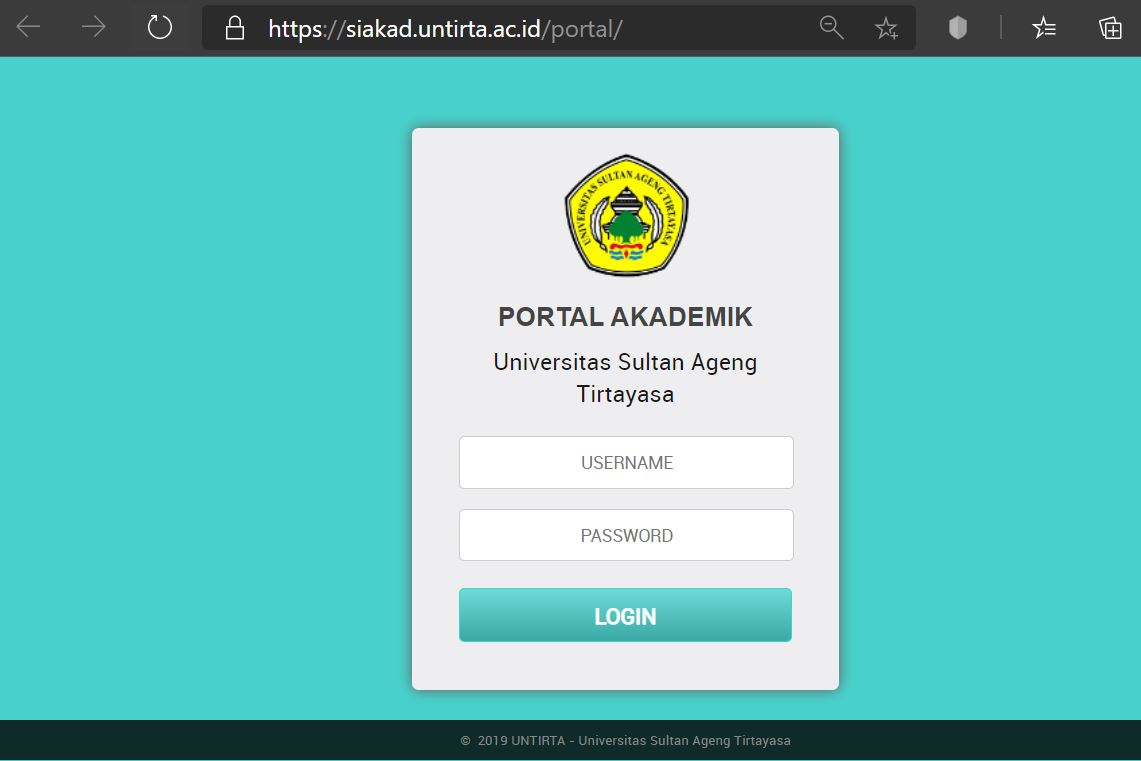
\includegraphics[width=8.33333in,height=\textheight]{static/3.1.JPG}

  Jika \emph{login} berhasil maka akan masuk ke halaman depan seperti berikut.

  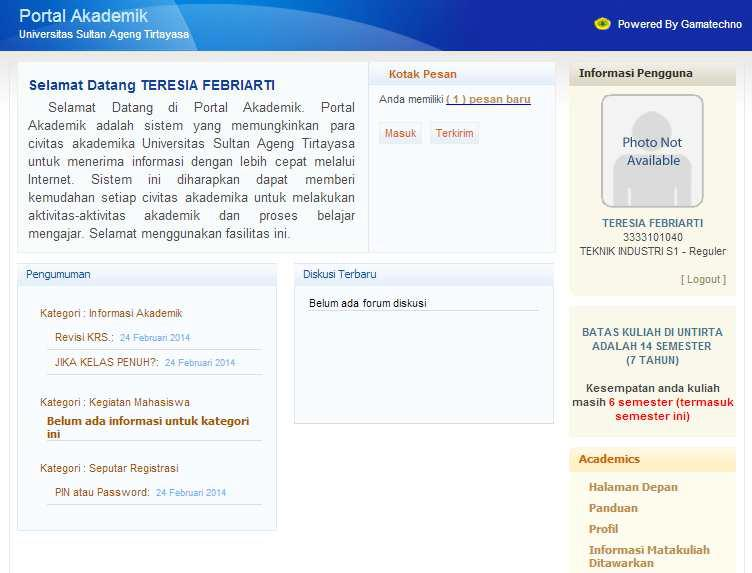
\includegraphics[width=8.33333in,height=\textheight]{static/3.2.jpg}

  \textbf{\emph{Profil mahasiswa}}

  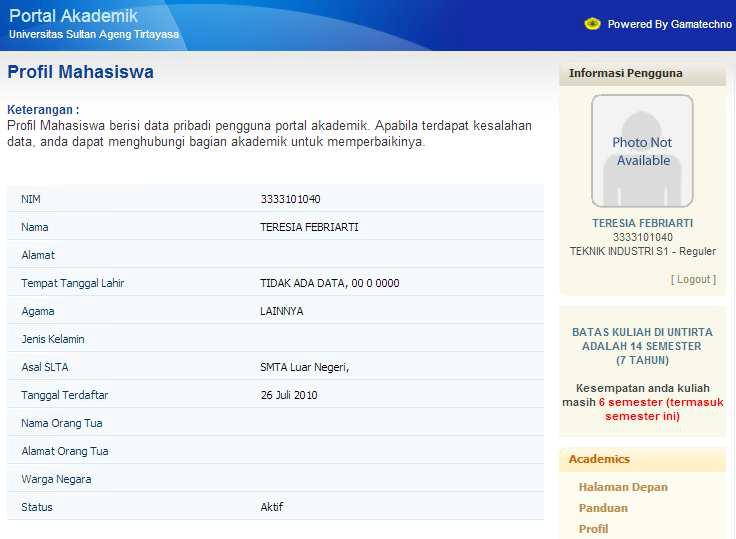
\includegraphics[width=8.33333in,height=\textheight]{static/3.3.jpg}

  \textbf{\emph{Informasi mata muliah yang ditawarkan}}

  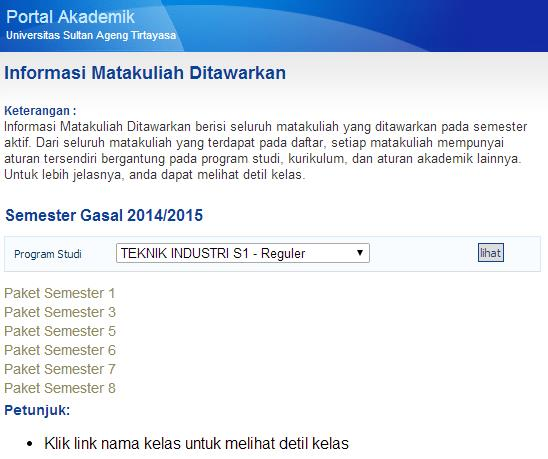
\includegraphics{static/3.4.jpg}

  Klik \textbf{Paket Semester} yang ada lalu klik kelas, nanti akan muncul detil kelas terkait kelas yang
  dibuka tersebut.

  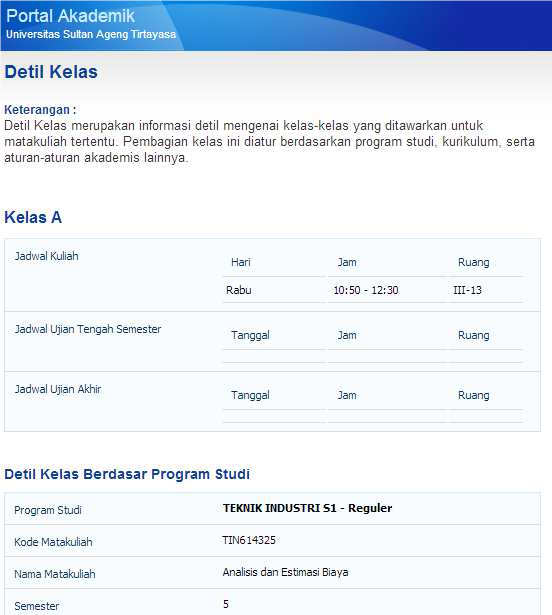
\includegraphics{static/3.5.png}

  \textbf{\emph{Kartu Rencana Studi}} \textbf{(\emph{KRS})}

  Lakukan kontrak mata kuliah sesuai petunjuk dan sesuai dengan Kartu Rencana Studi (KRS) yang sudah disetujui oleh Dosen pembimbing/Dosen Wali. Mengontrak Rencana Studi lalu mencetak Kartu Rencana Studi (KRS) adalah salah satu syarat bahwa mahasiswa tersebut aktif pada semester berjalan. Jika tidak melakukan KRS maka mahasiswa \textbf{Dianggap Tidak Aktif (Dicutikan).} KRS baru bisa dilakukan pada periode yang ditentukan oleh UPT. PUSDAINFO, dan jadwal kuliah sudah di-\emph{upload} oleh Program Studi.

  \begin{itemize}
  \item
    Klik Kartu Rencana Studi
  \item
    Klik Tambah Mata Kuliah
  \end{itemize}

  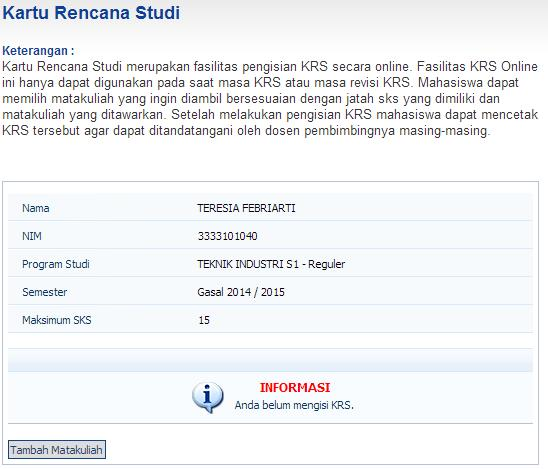
\includegraphics{static/3.6.jpg}

  Setelah muncul paket semesternya lalu:

  \begin{itemize}
  \item
    Klik paket semesternya
  \item
    Lalu pilih mata kuliah yang anda inginkan.
    (Catatan : bagi mahasiswa baru (tingkat 1), mata kuliah sudah paket dan kelasnya sudah ditentukan oleh Program Studi, maka sebaiknya tanyakan anda harus memilih mata kuliah apa dan kelasnya kelas apa.
  \item
    Setelah selesai memilih kelas, lalu klik Tambah
  \item
    Cetak KRS, lalu temui dosen Pembimbing Akademik untuk meminta persetujuan KRS.
  \item
    Copy kontrak mata kuliahnya atau \emph{print out} dan simpan sebagai dokumen pribadi.
  \end{itemize}

  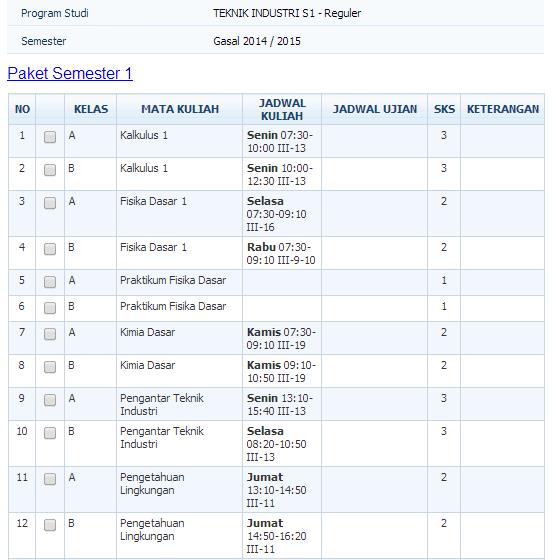
\includegraphics{static/3.7.jpg}

  \textbf{\emph{Kartu Hasil Studi}} \textbf{(\emph{KHS})}

  \begin{itemize}
  \item
    Pilih semester dimana anda ingin melihat hasil studi anda. Lalu klik lihat.
  \item
    Akan muncul seluruh mata kuliah dan nilai mata kuliah yang pernah anda ambil pada semester tersebut. Kemudian jika ingin mencetaknya silahkan klik cetak.
  \end{itemize}

  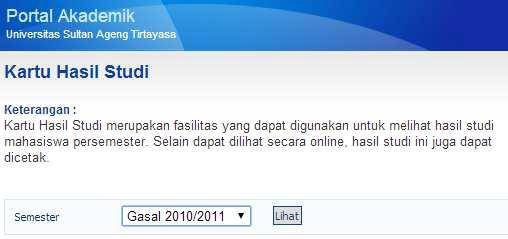
\includegraphics{static/3.8.jpg}

  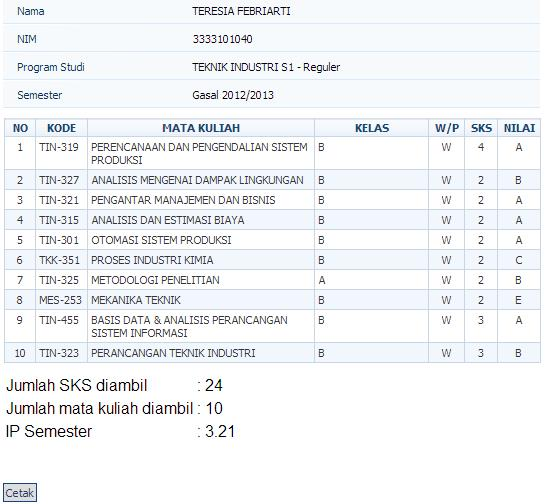
\includegraphics[width=5.29167in,height=\textheight]{static/3.81.jpg}

  \textbf{\emph{Transkrip Nilai}}

  Setelah diklik \textbf{Transkrip nilai}, seluruh nilai mata kuliah akan muncul sesuai kurikulum yang menjadi acuannya. Klik \textbf{cetak} jika ingin mencetak transkrip.

  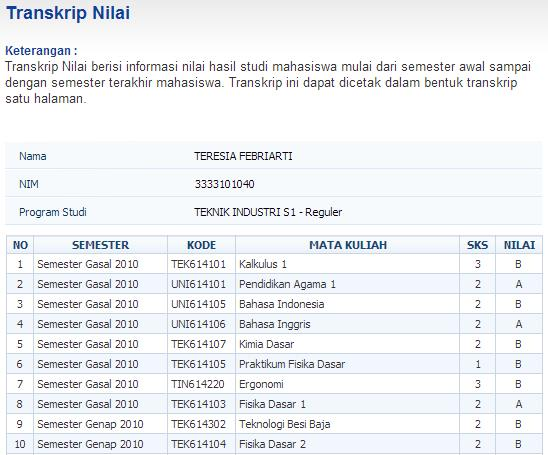
\includegraphics{static/3.9.jpg}

  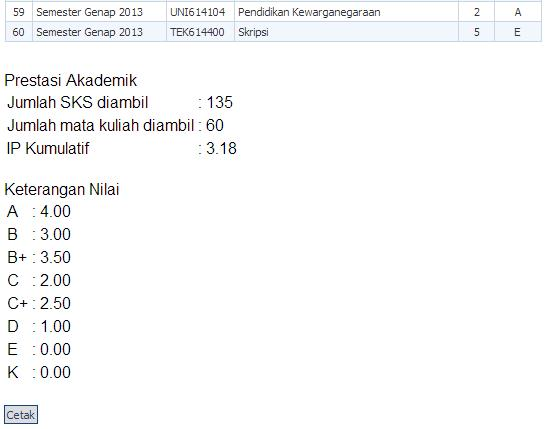
\includegraphics{static/3.91.jpg}

  \textbf{\emph{Mengubah Password}} \textbf{(\emph{Kode Akses})}

  Penting bagi mahasiswa untuk menjaga kerahasiaan \emph{password}. Gunakan \emph{password} yang gampang diingat dan tidak mudah ditebak oleh orang lain.

  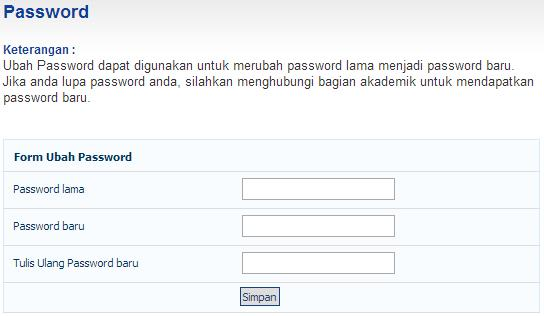
\includegraphics{static/3.92.jpg}

  \textbf{\emph{Berkirim Pesan}}

  Mahasiswa bisa berkirim pesan kepada seluruh mahasiswa dan dosen melalui portal akademik seperti berkirim email dengan alamat atau akun yang dituju adalah NIM mahasiswa dari orang yang akan dikirimkan pesan.
  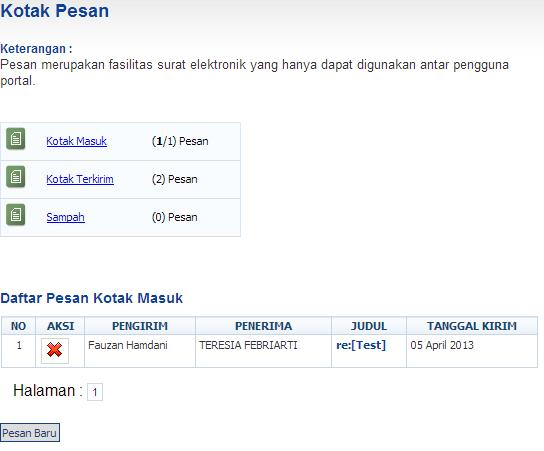
\includegraphics{static/3.93.jpg}
\item
  Mahasiwa melihat jadwal perkuliahan di fakultas untuk mengambil mata kuliah, dan dosen yang telah ditentukan oleh fakultas.
\item
  Kontrak mata kuliah/Pengambilan mata kuliah / Pengisian Kartu Rencana Studi (KRS), dicetak untuk diserahkan ke fakultas dan disetujui oleh dosen pembimbing / dosen wali, ditanda tangani, dan distempel fakultas.
\item
  Kartu Rencana Studi (KRS) diserahkan ke Pusat Data dan Informasi (PUSDAINFO).
\item
  Hasil Kartu Rencana Studi (KRS) \emph{online} dicetak untuk diserahkan ke fakultas/jurusan/program studi.
\end{enumerate}

\hypertarget{fakultasjurusanprogram-studi}{%
\subsubsection{Fakultas/Jurusan/Program Studi}\label{fakultasjurusanprogram-studi}}

Mahasiswa setelah melakukan registrasi \emph{online} /SIAKAD \emph{online} dan hasilnya kemudian dicetak untuk diserahkan ke fakultas/jurusan/program studi masing-masing untuk melakukan:

\begin{enumerate}
\def\labelenumi{\arabic{enumi}.}
\tightlist
\item
  Melakukan kontrak mata kuliah pada semester yang akan diambil.
\item
  Melakukan konsultasi bimbingan akademik dari wali akademik/dosen pembimbing untuk menyetujui mata kuliah yang akan diambil.
\item
  Mengisi Kartu Rencana Studi (KRS) dengan lengkap dan menyerahkan ke PUSDAINFO.
\end{enumerate}

\hypertarget{pusat-data-dan-informasi-pusdainfo}{%
\subsubsection{Pusat Data dan Informasi (PUSDAINFO)}\label{pusat-data-dan-informasi-pusdainfo}}

Pusat Data dan Informasi (PUSDAINFO) memproses Kartu Rencana Studi (KRS) dan diberikan kepada mahasiswa (dapat dilakukan oleh mahasiswa sendiri secara \emph{online}).

\hypertarget{mahasiswa-1}{%
\subsubsection{Mahasiswa}\label{mahasiswa-1}}

\begin{enumerate}
\def\labelenumi{\arabic{enumi}.}
\tightlist
\item
  Mendapatkan Kartu Rencana Studi (KRS) sesuai dengan mata kuliah yang dikontraknya.
\item
  Setelah mahasiswa mendapatkan Kartu Rencana Studi (KRS) dan namanya tercantum dalan Daftar Hadir Mahasiswa dan Dosen (DHMD), mahasiswa mengikuti perkuliahan sesuai mata kuliah yang dikontrak dalam Kartu Rencana Studi (KRS).
\end{enumerate}

\hypertarget{program-magister-s2-dan-doktor-s3}{%
\subsection{Program Magister (S2) dan Doktor (S3)}\label{program-magister-s2-dan-doktor-s3}}

Mahasiswa ProgramMagister \textbf{(}S2) dan Doktor (S3) dapat melakukan registrasi dengan melakukan prosedur sebagai berikut :

\begin{enumerate}
\def\labelenumi{\arabic{enumi}.}
\tightlist
\item
  Kontrak mata kuliah/Pengambilan mata kuliah, Mahasiswa mengisi Kartu Rencana Studi (KRS) di Bagian Akademik Pascasarjana.
\item
  Mahasiswa melakukan bimbingan mata kuliah ke dosen wali/dosen pembimbing di Pascasarjana, untuk disetujui dan ditandatangani serta distempel oleh Pascasarjana.
\item
  Mahasiswa melihat jadwal perkuliahan di Pascasarjana untuk mengambil mata kuliah, kelas, dan dosen, serta dosen pembimbing/dosen wali yang telah ditentukan oleh Pascasarjana.
\end{enumerate}

\hypertarget{petugas-registrasi}{%
\section{Petugas Registrasi}\label{petugas-registrasi}}

Petugas Registrasi yang terkait dalam pelaksanaan registrasi ulang mahasiswa lama antara lain:

\hypertarget{biro-akademik-kemahasiswaan-dan-perencanaan-bakp}{%
\subsection{Biro Akademik, Kemahasiswaan, dan Perencanaan (BAKP)}\label{biro-akademik-kemahasiswaan-dan-perencanaan-bakp}}

Biro Akademik, Kemahasiswaan, dan Perencanaan (BAKP) Universitas Sultan Ageng Tirtayasa melalui Subbagian Registrasi dan Statistik melaksanakan tugasnya melayani mahasiswa lama yang melakukan registrasi, mendokumentasikan laporan dan melakukan koordinasi dengan Subbagian Penerimaan Negara Bukan Pajak (PNBP), Pusat Data dan Informasi (PUSDAINFO), Jurusan/Prodi/Fakultas, Subbagian Akademik Pascasarjana, dan petugas bank yang ditunjuk (Bank BNI).

\hypertarget{biro-umum-keuangan-dan-kepegawaian-bukk}{%
\subsection{Biro Umum, Keuangan, dan Kepegawaian (BUKK)}\label{biro-umum-keuangan-dan-kepegawaian-bukk}}

Biro Umum, Keuangan, dan Kepegawaian (BUKK) Universitas Sultan Ageng Tirtayasa melaksanakan tugasnya sebagai biro yang menangani bidang keuangan melalui sub bagian Penerimaan Negara Bukan Pajak (PNBP) yang ditugaskan melayani mahasiswa lama yang melakukan registrasi, mendokumentasikan laporan dan melakukan koordinasi pada Subbagian Registrasi dan Statistik, Pusat Data dan Informasi (PUSDAINFO), Subbagian Kemahasiswaan, Subbagian Akademik Pascasarjana dan petugas bank yang ditunjuk yaitu Bank BNI perihal mahasiswa lama yang melakukan registrasi akademik dan mengadministrasikan/laporan registrasi mahasiswa baru yang melakukan pembayaran Uang Kuliah Tunggal (UKT) program Sarjana (S1) dan Diploma (D3) dan Sumbangan Pengembangan Pendidikan (SPP) Program Magister (S2).

\hypertarget{bank-bni}{%
\subsection{Bank BNI}\label{bank-bni}}

Melaksanakan tugasnya sebagai Bank yang ditunjuk oleh Universitas Sultan Ageng Tirtayasa sebagai Bank
yang menerima pembayaran mahasiswa lama yang melakukan registrasi yaitu : Uang Kuliah Tunggal (UKT) program Sarjana (S1) dan Diploma (D3) dan Sumbangan Pengembangan Pendidikan (SPP) Program
Magister (S2) dan Doktor (S3), melaksanakan koordinasi dengan Subbagian Penerimaan Negara Bukan Pajak (PNBP), Pusat Data dan Informasi (PUSDAINFO), dan Subbagian Registrasi dan Statistik.

\hypertarget{pusat-data-dan-informasi-pusdainfo-1}{%
\subsection{Pusat Data dan Informasi (PUSDAINFO)}\label{pusat-data-dan-informasi-pusdainfo-1}}

\begin{enumerate}
\def\labelenumi{\arabic{enumi}.}
\tightlist
\item
  Pusat Data dan Informasi (PUSDAINFO) menerima data mahasiswa lama yang melakukan registrasi dan yang telah mengisi Kartu Rencana Studi (KRS) dan mendapat bimbingan akademiknya, mahasiswa segera menyerahkan Kartu Rencana Studi (KRS) nya ke Pusat Data dan Informasi (PUSDAINFO) baik cetak maupun elektronik.
\item
  Mengolah data dan menerbitkan Kartu Rencana Studi (KRS) dan Daftar Hadir Mahasiswa dan Dosen (DHMD).
\item
  Mendokumentasikan laporan.
\item
  Melaksanakan koordinasi dengan Subbagian Penerimaan Negara Bukan Pajak (PNBP), Subbagian Registrasi dan Statistik, Jurusan/Program Studi, Fakultas, Subbagian Akademik Pascasarjana, dan petugas bank yang ditunjuk yaitu Bank BNI.
\end{enumerate}

\hypertarget{jurusanprogram-studi}{%
\subsection{Jurusan/Program Studi}\label{jurusanprogram-studi}}

Jurusan/Program Studi menerima data mahasiswa lama yang telah melakukan registrasi dan melakukan
Kartu Rencana Studi (KRS) membuat jadwal perkuliahan dan Daftar Hadir Mahasiswa dan Dosen (DHMD).

\hypertarget{pascasarjana}{%
\subsection{Pascasarjana}\label{pascasarjana}}

\begin{enumerate}
\def\labelenumi{\arabic{enumi}.}
\tightlist
\item
  Subbagian Akademik Pascasarjana menerima data mahasiswa yang telah mengisi pada Kartu Rencana Studi (KRS) dan mendapat bimbingan akademiknya, mahasiswa segera menyerahkan Kartu Rencana
  Studi (KRS) nya ke Subbagian Akademik Pascasarjana.
\item
  Mengolah data dan menerbitkan Kartu Rencana Studi (KRS) dan Daftar Hadir Mahasiswa dan Dosen (DHMD).
\end{enumerate}

\hypertarget{pascasarjanafakultas}{%
\subsection{Pascasarjana/Fakultas}\label{pascasarjanafakultas}}

Mengendalikan operasional jalannya kegiatan perkuliahan sesuai dengan jadwal perkuliahan yang telah ditentukan.

\begin{figure}
\centering
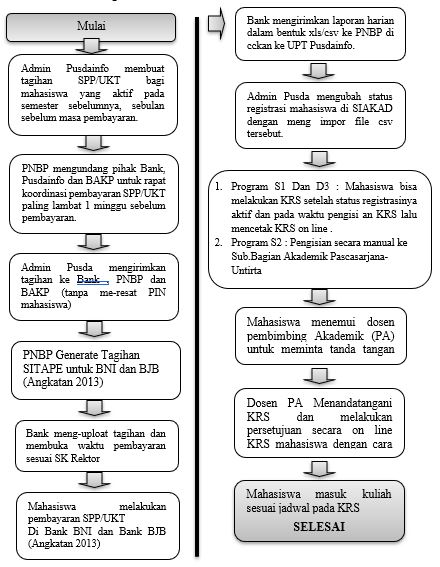
\includegraphics{static/3.94.JPG}
\caption{Flowchart registrasi mahasiswa lama}
\end{figure}

\hypertarget{pengajuan-ijin-cuti-kuliah}{%
\chapter{PENGAJUAN IJIN CUTI KULIAH}\label{pengajuan-ijin-cuti-kuliah}}

\hypertarget{ketentuan-pengajuan-cuti-kuliah}{%
\section{Ketentuan Pengajuan Cuti Kuliah}\label{ketentuan-pengajuan-cuti-kuliah}}

\hypertarget{waktu-registrasi}{%
\section{Waktu Registrasi}\label{waktu-registrasi}}

\hypertarget{prosedur-pengajuan-cuti-kuliah}{%
\section{Prosedur Pengajuan Cuti Kuliah}\label{prosedur-pengajuan-cuti-kuliah}}

\hypertarget{petugas-registrasi}{%
\section{Petugas Registrasi}\label{petugas-registrasi}}

\hypertarget{pengajuan-aktif-kuliah-kembali}{%
\chapter{PENGAJUAN AKTIF KULIAH KEMBALI}\label{pengajuan-aktif-kuliah-kembali}}

\hypertarget{ketentuan-pengajuan-aktif-kuliah-kembali}{%
\section{Ketentuan Pengajuan Aktif Kuliah Kembali}\label{ketentuan-pengajuan-aktif-kuliah-kembali}}

\hypertarget{waktu-registrasi}{%
\section{Waktu Registrasi}\label{waktu-registrasi}}

\hypertarget{prosedur-pengajuan-aktif-kuliah-kembali}{%
\section{Prosedur Pengajuan Aktif Kuliah Kembali}\label{prosedur-pengajuan-aktif-kuliah-kembali}}

\hypertarget{prosedur-kontrak-mata-kuliah}{%
\section{Prosedur Kontrak Mata Kuliah}\label{prosedur-kontrak-mata-kuliah}}

\hypertarget{petugas-registrasi}{%
\section{Petugas Registrasi}\label{petugas-registrasi}}

\hypertarget{pengajuan-pindah-program-studi}{%
\chapter{PENGAJUAN PINDAH PROGRAM STUDI}\label{pengajuan-pindah-program-studi}}

\hypertarget{ketentuan-umum-pengajuan-pindah-program-studi}{%
\section{Ketentuan Umum Pengajuan Pindah Program Studi}\label{ketentuan-umum-pengajuan-pindah-program-studi}}

\hypertarget{waktu-registrasi}{%
\section{Waktu Registrasi}\label{waktu-registrasi}}

\hypertarget{prosedur-pengajuan-pindah-program-studi}{%
\section{Prosedur Pengajuan Pindah Program Studi}\label{prosedur-pengajuan-pindah-program-studi}}

\hypertarget{prosedur-kontrak-mata-kuliah}{%
\section{Prosedur Kontrak Mata Kuliah}\label{prosedur-kontrak-mata-kuliah}}

\hypertarget{petugas-registrasi}{%
\section{Petugas Registrasi}\label{petugas-registrasi}}

\hypertarget{pengajuan-pindah-kuliah-ke-pt-lain}{%
\chapter{PENGAJUAN PINDAH KULIAH KE PT LAIN}\label{pengajuan-pindah-kuliah-ke-pt-lain}}

\hypertarget{ketentuan-umum-pengajuan-pindah-kuliah-ke-pt-lain}{%
\section{Ketentuan Umum Pengajuan Pindah Kuliah ke PT Lain}\label{ketentuan-umum-pengajuan-pindah-kuliah-ke-pt-lain}}

\hypertarget{waktu-registrasi}{%
\section{Waktu Registrasi}\label{waktu-registrasi}}

\hypertarget{prosedur-pengajuan-pindah-kuliah-keluar-dari-untirta}{%
\section{Prosedur Pengajuan Pindah Kuliah (Keluar dari Untirta)}\label{prosedur-pengajuan-pindah-kuliah-keluar-dari-untirta}}

\hypertarget{petugas-registrasi}{%
\section{Petugas Registrasi}\label{petugas-registrasi}}

\hypertarget{permohonan-pernyataan-masih-kuliah}{%
\chapter{PERMOHONAN PERNYATAAN MASIH KULIAH}\label{permohonan-pernyataan-masih-kuliah}}

\hypertarget{ketentuan-pengajuan-surat-pernyataan-masih-kuliah}{%
\section{Ketentuan Pengajuan Surat Pernyataan Masih Kuliah}\label{ketentuan-pengajuan-surat-pernyataan-masih-kuliah}}

\hypertarget{waktu-registrasi}{%
\section{Waktu Registrasi}\label{waktu-registrasi}}

\hypertarget{prosedur-pengajuan-surat-pernyataan-masih-kuliah}{%
\section{Prosedur Pengajuan Surat Pernyataan Masih Kuliah}\label{prosedur-pengajuan-surat-pernyataan-masih-kuliah}}

\hypertarget{alih-jenjang}{%
\chapter{ALIH JENJANG}\label{alih-jenjang}}

\hypertarget{dari-luar-ke-untirta}{%
\section{Dari Luar ke Untirta}\label{dari-luar-ke-untirta}}

\hypertarget{d3-feb-ke-s1}{%
\section{D3 FEB ke S1}\label{d3-feb-ke-s1}}

  \bibliography{book.bib,packages.bib}

\end{document}
